\documentclass{beamer}
\usepackage{bm}
\usepackage{mathtools}
\DeclarePairedDelimiter{\norm}{\lVert}{\rVert}
\usepackage{esdiff}
\usepackage{amsthm}
%\newtheorem{def}{Definition}
%\usepackage{graphicx}
%\mode{presentation}
\title{Signal Processing Techniques for Interpolation in Graph Structured Data}
\author{Reporter: Feng Zhao\\Department of Electronic Engineering}
\begin{document}
\begin{frame}
\titlepage
\end{frame}
\begin{frame}
\frametitle{An example of recommendation system}
\begin{columns}
\column{0.5\textwidth}
\begin{itemize}
\item Five movies
\item a $5\times 5$ similarity matrix
\item a user rating on movie 1,2,5
\item predict his rating on movie 3,4 
\end{itemize}
\column{0.5\textwidth}
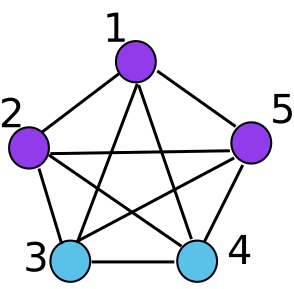
\includegraphics[width=0.5\textwidth]{movie5.eps}
\end{columns}
\end{frame}

\begin{frame}
\frametitle{kNN Method to predict user rating on movies}
\begin{columns}
\column{0.5\textwidth}
\begin{itemize}
\item predict on movie 3
\item suppose k=2
\item movie 2 and 5 are more similar to 3 than 1
\item predicted rating on movie 3: $\frac{1.2\times 4+0.8\times 2}{1.2+0.8}$
\end{itemize}
\column{0.5\textwidth}
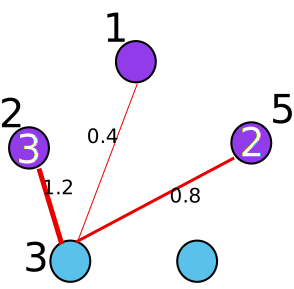
\includegraphics[width=0.5\textwidth]{movie5_knn.eps}
\end{columns}
\end{frame}

\begin{frame}
\frametitle{issues of kNN}
\begin{columns}
\column{0.5\textwidth}
\begin{itemize}
\item discard mutual information between movie 1,2,5
\item predict rating 3,4 respectively
\item jointly prediction with all information used will improve the \textit{accuracy} but also increase the \textit{complexity}.
\end{itemize}
\column{0.5\textwidth}
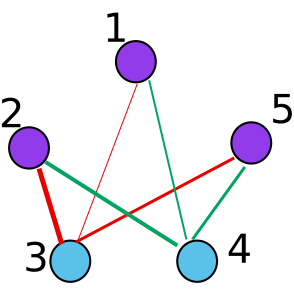
\includegraphics[width=0.5\textwidth]{movie5_knn_issues.eps}
\end{columns}
\end{frame}

\begin{frame}
\frametitle{Problem Reformulation}
\begin{columns}
\column{0.5\textwidth}
\begin{itemize}
\item $f(1),f(2),f(5)$ are known
\item \textit{interpolate} $f(3),f(4)$
\item $\bm{f}=[f(1),f(2),f(3),f(4),f(5)]^T$
\item $\bm{f}=f(1)\bm{\Theta}_1 + f(2)\bm{\Theta}_2 + f(5)\bm{\Theta}_5$
\end{itemize}
What is the space spanned by $\bm{\Theta}_1,\bm{\Theta}_2,\bm{\Theta}_5$?
\column{0.5\textwidth}
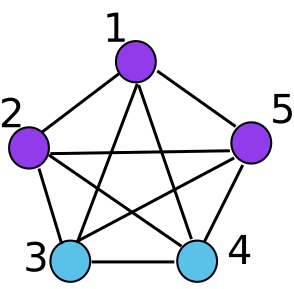
\includegraphics[width=0.5\textwidth]{movie5.eps}
\end{columns}
\end{frame}

\begin{frame}
\frametitle{band limited graph signal reconstruction}
\begin{block}{Nyquist Shannon sampling theorem}
If a continuous signal is band-limited, it can be reconstructed by discrete sampling without loss.
\end{block}
\begin{block}{Pesenson, Isaac}
If a graph signal is band-limited, it is uniquely determined by their values on some sets of vertices.
\end{block}
\end{frame}
%% remove these frames as they are unnecessary
%\begin{frame}
%\frametitle{band limited graph signal space}
%\begin{block}{continuous periodical case}
%\begin{enumerate}
%\item The signal is reconstructed in frequency domain. 
%\item $\{g_n\}$ is an orthogonal basis on $[0,2\pi]$ 
%\item $f(x)=\displaystyle\sum_{n=-\infty}^{\infty} \omega_ng_n(x)$, the frequency representation is $\{\omega_n\}$
%\end{enumerate}
%\end{block}
%\begin{block}{discrete case}
%If we have an orthogonal basis $g_n,n=1,2\dots,N$, then $f=\displaystyle\sum_{n=1}^{N} \omega_n g_n$
%\end{block}
%\end{frame}

%\begin{frame}
%\frametitle{How to get a set of orthogonal basis}
%\begin{block}{Sturm-Liouville theory}
%The solution to 
%\begin{equation}
%\diff[2]{y}{x}+y=-\lambda y,x\in[0,2\pi]
%\end{equation}
%gives an orthogonal basis $g_n(x),s.t. \mathcal{L}g=\lambda g$, where $\mathcal{L}$ is the Laplace operator.
%\begin{enumerate}
%\item $\mathcal{L}g=\diff[2]{g}{x}$ 
%\item $\mathcal{L}g=\diffp{g}{{x^2}}+\diffp{g}{{y^2}}$
%\end{enumerate}
%\end{block}
%Laplace operator $\Rightarrow$ Eigen-Problems 
%\end{frame}
%\begin{frame}
%\frametitle{Discrete Laplace operator}
%\begin{block}{geometric meaning of Laplace operator}
%divergence of gradient (vector field)
%\end{block}
%\begin{figure}
%\includegraphics[width=\textwidth]{div1d.eps}
%\caption{vector field $\nabla f$ over real line}
%\end{figure}
%$$
%\mathcal{L}f(x)=\frac{1}{2\Delta x}[\nabla f(x+\Delta x)-\nabla f(x-\Delta x)],\textrm{as } \Delta x\to 0
%$$
%\begin{itemize}
%\item divergence at $A$ is negative. 
%\item divergence at $B$ is zero
%\item divergence at $C$ is positive.
%\end{itemize}
%\end{frame}
%\begin{frame}
%\frametitle{Discrete Laplace operator}
%\begin{block}{1D case}
%\begin{align*}
%\mathcal{L}^d (f)(x_0) & = \frac{1}{h}[\nabla f(x_0+\frac{1}{2}h)-\nabla f(x_0-\frac{1}{2}h)] \\
%& = \frac{1}{h^2} [f(x_0+h)-f(x_0)+f(x_0-h)-f(x_0)]
%\end{align*}
%\end{block}
%\begin{block}{2D case}
%In grid lattice, the discrete laplace operator:
%$$
%\mathcal{L}^d (f)(\bm{P}_0) = \frac{1}{h^2} \sum_{\bm{P}\in \mathcal{N}_{\bm{P}_0}}(f(\bm{P})-f(\bm{P}_0))
%$$
%\end{block}
%\vspace{-1cm}
%\begin{block}{generalization to graph}
%$$
%\mathcal{L}^d (f)(\bm{P}_0) = \frac{1}{h^2} \sum_{\bm{P}\in \mathcal{N}_{\bm{P}_0}}w_{\bm{PP}_0}(f(\bm{P})-f(\bm{P}_0))
%$$
%\end{block}
%\end{frame}
%\begin{frame}
%\begin{definition}[Band Limited Signal]
%$\norm{\mathcal{L}^d (f)}\leq \omega_0 \norm{f}$
%\end{definition}
%\end{frame}
\begin{frame}
\frametitle{Reconstruction from basis}
\begin{block}{Critial Frequency}
If the graph signal is band-limited, its spectrum decomposition has only components less than critical frequency $\omega^*_S$.
\begin{equation}
 \bm{f} = \sum_{i}x_i\bm{v}_i
\end{equation}
where $\bm{v}_i$ is the eigenvector with eigenvalues less than $\omega^*_S$.
\end{block}
\begin{block}{Least Square}
\end{block}
$\bm{f}$ known only partially, least square techinque can be used to solve $x_i$

\end{frame}
\begin{frame}
\frametitle{Numerical Results}
\begin{block}{Dataset}
\begin{itemize}
\item Student body test data with 488 records and 37 features.
\item Use other features(excluding age) to predict the gender
\item 80\% training set, 20\% test set, 5 fold cross validation
\end{itemize}
\end{block}
\begin{block}{Algorithm}
\begin{itemize}
\item \textbf{Linear Discrimant Analysis} with average error rate at 0.4\%
\item \textbf{Graph Interpolation} with average error rate at 3\%
\end{itemize}
\end{block}
\end{frame}
\begin{frame}
\frametitle{Problems for Graph Interpolation}
\begin{itemize}
\item Edge weight from data features
\item Heuristic critical frequency
\end{itemize}
\end{frame}
\begin{frame}
\frametitle{Acknowledgement}
\begin{center}
\itshape\Huge Thanks for listening
\end{center}
\end{frame}

\end{document}
